\subsubsection{Progressió de la cerca}

\paragraph{}
Un dels aspectes d'usabilitat més interessants d'aquesta funcionalitat és la secció dedicada a mostrar la progressió de la cerca. Si ja havíem comentat que a mesura que es reben les dades dels diferents anys, aquestes són representades en els gràfics pertinents, aquesta secció de la pàgina compleix un rol similar, però més informatiu.

En el moment que es llança una cerca, l'usuari és transportat a aquesta secció. Durant el temps de cerca, aquesta secció mostra el cognom pel qual s'està realitzant la cerca, la duració estimada calculada mitjançant la fórmula: \emph{númeroPaïsos} $\times$ \emph{númeroAnys} $\times$ \emph{apiDELAY}, la informació sobre el país i any dels quals s'està esperant la resposta per part del SDK i una barra del progrés actual, respecta el total estimat.

Una cosa que cal tenir en compte és que les crides al SDK són asíncrones i que per tant, no està garantit que el retorn d'aquestes segueixi el mateix ordre que l'ordre d'enviament. Això significa, que potser, el bloc HTML que mostra la progressió de la cerca, pot indicar que s’estan esperant dades que ja han arribat o viceversa. De totes maneres, s’espera que en la gran majoria dels casos, hi hagi una correlació entre l’ordre d’enviament i retorn de les peticions al SDK.

En qualsevol cas, el fet més important relatiu a la barra de progrés, és que aquesta arribi al 100\% quan s'han processat totes les crides a l’API i que cada crida emmagatzemi el resultat a les caselles de la matriu que li pertoca. Recordem que això és aconseguit gràcies als paràmetres \emph{i} i \emph{k}, encapsulats en les crides.

Quan la cerca és completada, canvia l'estat dels components de la secció i s'indica que la cerca ha estat completada pel cognom especificat, s'elimina el temps estimat de finalització i és substituït per una indicació sobre la localització dels resultats i s'indica el nombre total de països i anys cercats. L'efecte de moviment en la barra de progressió, també és eliminat, per tal d'evitar confondre a l'usuari.

La imatge\ref{fig:waitingSurnames} mostra dos estats diferents de la secció progressió de la cerca.

\begin{figure}
    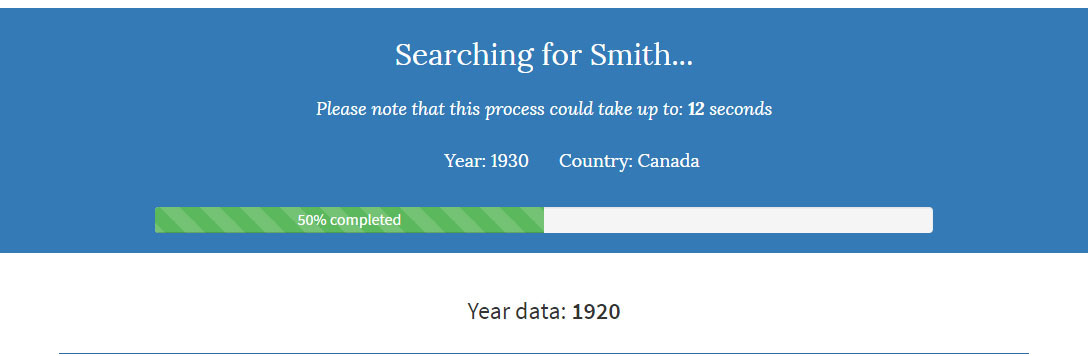
\includegraphics[width=\linewidth]{11/03_surnamesSearch/06_waitingDesktop}
    
\includegraphics[width=\linewidth]{11/03_surnamesSearch/07_waitingDesktopComplete}
    \centering
    \caption{Exemples de la secció progressió de la cerca}\label{fig:waitingSurnames}
\end{figure}
